\documentclass[12pt, twoside]{article}
\usepackage[letterpaper, margin=1in, headsep=0.5in]{geometry}
\usepackage[english]{babel}
\usepackage[utf8]{inputenc}
\usepackage{amsmath}
\usepackage{amsfonts}
\usepackage{amssymb}
\usepackage{tikz}
%\usetikzlibrary{quotes, angles}

\usepackage{graphicx}
\usepackage{enumitem}
\usepackage{multicol}

\usepackage{fancyhdr}
\pagestyle{fancy}
\fancyhf{}
\renewcommand{\headrulewidth}{0pt} % disable the underline of the header

\fancyhead[RE]{\thepage}
\fancyhead[RO]{\thepage \\ Name: \hspace{3cm}}
\fancyhead[L]{BECA / Dr. Huson / Geometry\\* 31 January 2019}

\begin{document}
\subsubsection*{7-3 Do Now: Graphing linear equations}
  \begin{enumerate}

\item Graph and label the two equations. Mark their intersection as an ordered pair.

  \begin{multicols}{2}
    $y = -2x-1$ \\
    $2x+3y = 9$
  \end{multicols}
  Are the lines parallel, perpendicular, or neither? Justify your answer.
  \vspace{1.5cm}

  \begin{center} %4 quadrant regents grid w T-Chart
  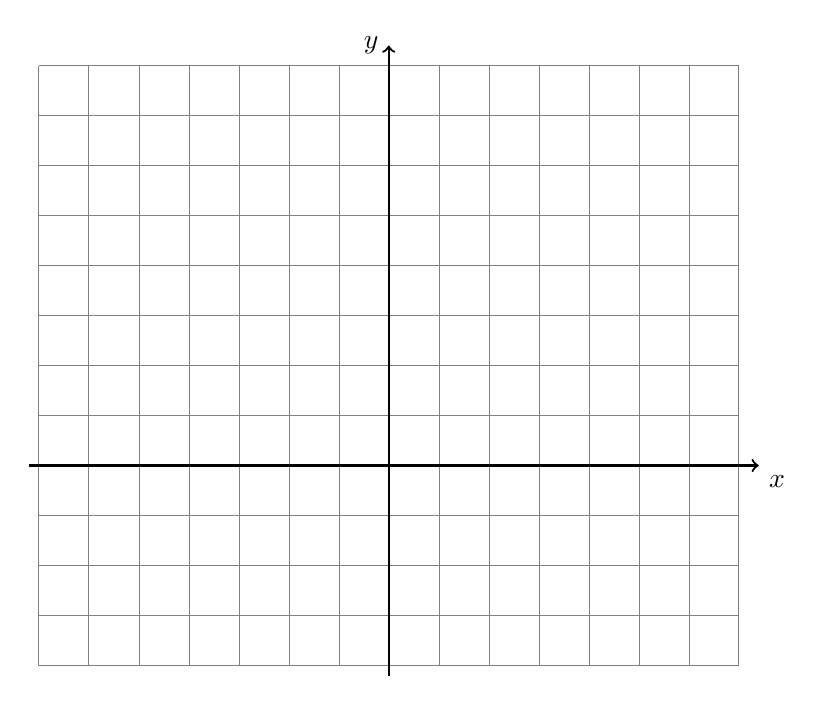
\begin{tikzpicture}[scale=.635]
    \draw [help lines] (-7,-4) grid (7,8);
    \draw [thick, ->] (-7.2,0) -- (7.4,0) node [below right] {$x$};
    \draw [thick, ->] (0,-4.2)--(0,8.4) node [left] {$y$};
  \end{tikzpicture}
  \end{center}


    \item A translation of $x \rightarrow x-4, y \rightarrow y-3$ maps $\overline{AB} \rightarrow \overline{CD}$, with $A(0,2)$ and $B(4,0)$. Find the slopes and $y$-intercepts of $\overleftrightarrow{AB}$ and $\overleftrightarrow{CD}$, and hence write down the equations of the two lines.

  \end{enumerate}
  \setcounter{page}{1}
  \newpage
\subsubsection*{7-3 Homework: Quadratic functions}
Show your work. For graphs, use a pencil and straight edge.
  \begin{enumerate}

\item Graph and label each function. Mark the vertices as ordered pairs and the $x$- and $y$-intercepts with their values.
        \vspace{0.25cm}
        \begin{multicols}{2}
          $f(x)=x^2$\\
          $g(x)=(x-3)^2-4$
        \end{multicols}
        What transformation maps $f$ onto $g$?
        \vspace{2.25cm}

    \begin{center} %4 quadrant regents grid w T-Chart
    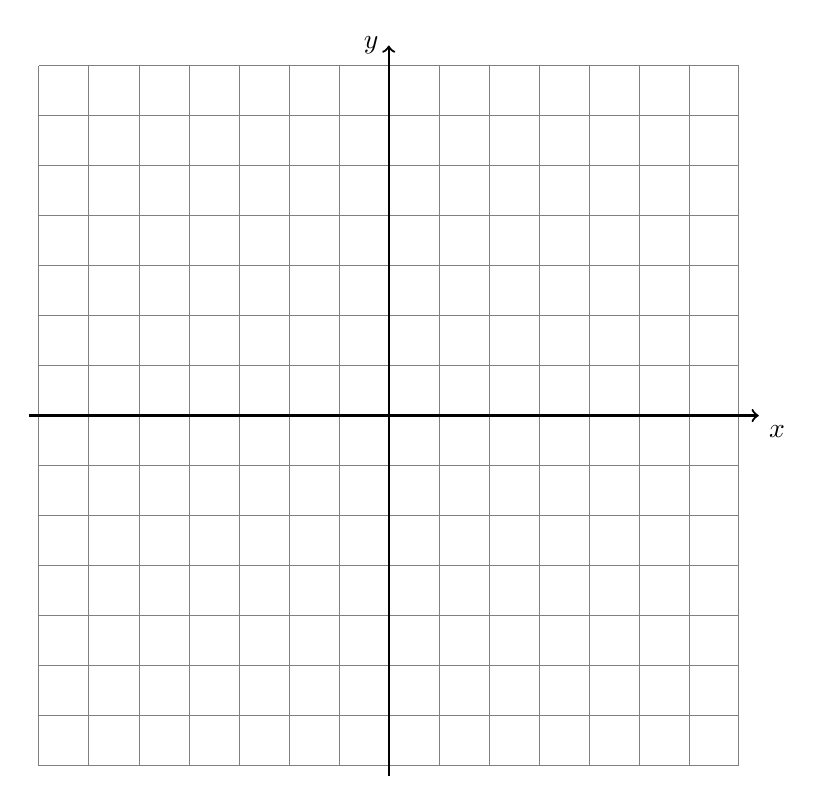
\begin{tikzpicture}[scale=.635]
      \draw [help lines] (-7,-7) grid (7,7);
      \draw [thick, ->] (-7.2,0) -- (7.4,0) node [below right] {$x$};
      \draw [thick, ->] (0,-7.2)--(0,7.4) node [left] {$y$};
    \end{tikzpicture}
    \end{center}


    In the following two problems, solve for the value of $x$.
    \begin{multicols}{2}
    \item   $\frac{3}{7}(14+21x)=-3$ \vspace{3cm}
    \item   $\frac{1}{4}(5-3x)=-1$ \vspace{3cm}
    \end{multicols}

\newpage

\item Given $f(x)=x^2-2x+1$. Simplify $f(0)$. \vspace{2cm}
\item Given $g(x)=\frac{2}{3} x+2$. Solve for $x$ such that for $g(x)=6$. \vspace{2.5cm}
\item Solve $x^2-6x+5=0$. \vspace{3cm}

\item The line $\overleftrightarrow{PQ}$ has the equation $2x+5y=10$ with the two points' coordinates $P(0,a)$ and $Q(b,0)$. Find the values of $a$ and $b$. \vspace{5cm}

Factor each quadratic
\begin{multicols}{2}
  \item $f(x)=x^2-6x+9$ \vspace{3.5cm}
  \item $g(x)=x^2+7x+12$ \vspace{3cm}
\end{multicols}


\end{enumerate}

\end{document}
